\documentclass{school-22.101-notes}
\date{October 12, 2011}

\begin{document}
\maketitle

%%%%%%%%%%%%%%%%%%%%%%%%%%% Angular Momentum %%%%%%%%%%%%%%%%%%%%
\lecture{Angular Momentum}
Angular momentum is a conserved quantity in a central force field. While a general potential is dependent on the spatial coordinate:
\eqn{ V(\uline{x}) = V(r,\theta, \phi)   }
a special potential that is only depend on radius (no $\theta, \phi$ dependency) is called a central force field because of its rotational symmetry. 

Section.~\ref{section-physical-angular-momentum} through \ref{section-Pauli} were given on Oct. 1-3, 2012 by Prof. Ju Li. 

%%%%%%%%%%%%%%% 12 Fall %%%%%%%%%%%%%%%%%
\topic{Physical Meaning of Momenta \label{section-physical-angular-momentum}}
\hi{Momentum is a generator of translation.} Consider an operator $T$ that transforms $\psi(x)$ to $\psi(x-\Delta x)$: 
\eqn{ T \psi(x) = \psi(x-\Delta x)} 
We perform the Taylor expansion on $\psi(x - \Delta x)$: 
\begin{align}
  \psi(x - \Delta x) &= \psi(x) + (-\Delta x) \ppsipx + \frac{(-\Delta x)^2}{2!} \ppsipxn2 + \frac{(-\Delta x)^3}{3!} \ppsipxn3 + \cdots \\
  &= \left[ 1 - \Delta x \ppx + \frac{(-\Delta x \ppxn2)^2}{2!} + \frac{(-\Delta x \ppxn3)^3}{3!} + \cdots \right] \psi(x) 
\end{align}
Using $e^x = 1 + x + \frac{x^2}{2!} + \frac{x^3}{3!} + \cdots$, we can write, 
\begin{align}
  \psi(x - \Delta x) &= \exp \left( -\Delta x \ppx \right) \psi(x) \\
  &= \exp \left(- \frac{i \Delta x (-i \hbar \ppx)}{\hbar} \right) \psi(x) \\
  &= \exp \left(-\frac{i \Delta x \cdot \hat{P} }{\hbar} \right) \psi(x) \label{momentum-meaning}
\end{align}

Eq.~\ref{momentum-meaning} implies that the position transform vector is the momentum operator. 


\hi{Angular momentum is a generator of rotation.} We consider an operator $R(n, \theta)$ that rotate a $\psi$ to $\psi_{\mathrm{rot}}$: 
\eqn{ R(\vec{n}, \theta) \psi = \psi_{\mathrm{rot}} }
We can prove that 
\eqn{ R(\vec{n}, \theta) = \exp \left( - \frac{i \theta}{\hbar} \vec{n} \cdot \vec{J} \right) \label{scalar-R} }
where $\vec{n}$ is the axis of rotation, $\theta$ is the amount of rotation in radian.  Keep in mind this $R(\vec{n}, \theta)$ is a scalar operator. 


\topic{Properties of Angular Momenta}
Now we are going to approach a measurement of an arbitrary vector operator $V$(the vector notation is ommited in this section) from two angles:
\begin{enumerate}
\item Recall the expression for $R(\vecn, \theta)$ in Eq.~\ref{scalar-R}. Then for an arbitrary vector operator $V$, a measurement can be written as, 
\eqn{ \bra{\psi} R^+ V R \ket{\psi} &= \bra{\psi} \exp \left( \frac{i \theta \vec{n} \cdot \vec{J} }{\hbar} \right) V \exp \left( - \frac{i \theta \vec{n} \cdot \vec{J} }{\hbar} \right) \ket{\psi}   \label{mom-phy-ang} }
For small $\theta$, we can Taylor expand the RHS of Eq.~\ref{mom-phy-ang}, 
\eqn{ \exp \left( \frac{i \theta \vec{n} \cdot \vec{J} }{\hbar} \right) V \exp \left( - \frac{i \theta \vec{n} \cdot \vec{J} }{\hbar} \right) = V + \frac{i \theta}{\hbar} [\vec{n} \cdot \vec{j}, V] + O(\theta^2) }
That is, the measurement becomes, 
\eqn{ \bra{\psi} V + \frac{i \theta}{\hbar} [\vec{n} \cdot \vec{j}, V] \ket{\psi}  \label{measurement-1} }

\item If we prepare a $\psi_{\mathrm{rot}}$, measure the expectation of $V$, the result should be a rotated version of expectation of the original measurement. That is, there is a 3x3 rotation matrix (matrix of numbers, not operators) with the following property: 
\eqn{ \bra{\psi_{\mathrm{rot}}} V \ket{\psi_{\mathrm{rot}}} &= \vec{R}(\vec{n}, \theta) \bra{\psi} V \ket{\psi}  }
Again we Taylor expand for small $\theta$, 
\eqn{ \vec{R} (\vecn, \theta) V = V + \theta (\vec{n} \cross V ) + O (\theta^2) }
The the measurement becomes, 
\eqn{ \bra{\psi} V + \theta (\vec{n} \cross V ) \ket{\psi}  \label{measurement-2}  }
\end{enumerate}
The two ways should yield same result, so we can equate Eq.~\ref{measurement-1} and Eq.~\ref{measurement-2}: 
\begin{align}
\bra{\psi} V + \frac{i \theta}{\hbar} [\vec{n} \cdot \vec{j}, V] \ket{\psi}  &=  \bra{\psi} V + \theta (\vec{n} \cross V ) \ket{\psi} \\
\bra{\psi}  \frac{i \theta}{\hbar} [\vec{n} \cdot \vec{j}, V] \ket{\psi}  &=  \bra{\psi} \theta (\vec{n} \cross V ) \ket{\psi} \\
\bra{\psi}  \frac{i}{\hbar} [\vec{n} \cdot \vec{j}, V] \ket{\psi}  &=  \bra{\psi} \vec{n} \cross V \ket{\psi} \\
\bra{\psi} \frac{i}{\hbar} [n_j J_j, V] \ket{\psi}  &= \vec{n} \cross \bra{\psi} V \ket{\psi} \\
\bra{\psi} \frac{i}{\hbar} [n_j J_j, V_i] \ket{\psi} &= \epsilon_{i,j,k} n_j \bra{\psi} V_k \ket{\psi} \\
\frac{i}{\hbar} [J_j, V_i] &= \epsilon_{ijk} V_k \\
\Aboxed{ [V_i, J_j] &= i \hbar \epsilon_{ijk} V_k }  \label{J-basic}
\end{align}

Recall that $[\vec{x}, \vec{P} ] = i \hbar \epsilon_{ijk} V_k$. Thus, the angular momentum (really the orbital angular momentum $\vec{L}$ as we haven't discuss spin yet) is, 
\eqn{ \Aboxed{ \vec{L} &= \vec{x} \cross \vec{P}  } \label{defn-J} }

\clearpage
Now that we know some fundamental properties of $\vec{J}$, we can do the following to make use of them.
\begin{enumerate}
\item We define a $J^2$ term,
  \eqn{ J^2 &= \vec{J} \cdot \vec{J} = J_x^2 + J_y^2 + J_z^2 = J_i J_i }
  Using $[AB,C] = A[B,C] + [A,C] B$, 
  \eqn{ [J^2, J_3] &= [J_i J_i, J_3] = J_i [J_i, J_3] + [J_i, J_3] J_i }
  Apply Eq.~\ref{J-basic} on the $[J_i, J_3]$ terms,
  \eqn{ [J^2,J_3] &= J_i (i \hbar \epsilon_{i3k} J_k) + (i\hbar \epsilon_{i3k} J_k) J_i  = i\hbar \epsilon_{i3k} (J_i J_k + J_k J_i) = 0 }
  Basically \hi{$J^2$ commutes with any projection of $J$}, 
  \eqn{ \boxed{ [J^2, \vecn \cdot \vec{J} ] = [J^2, n_x J_x + n_y J_y + n_z J_z] = 0}  }
  which includes, 
  \eqn{ [J^2, J_x] &= 0,  & [J^2, J_y] &=0, &[J^2, J_z]&=0, & [J^2,J_+]&=0, & [J^2, J_-]&= 0 }

\item We define the raising operator $J_+ = J_x + iJ_y$, and the lowering operator $J_- = J_x - iJ_y$. As we've seen above, $[J^2, J_+] = [J^2, J_-] = 0$. Next we show how $J_+, J_-$ relate to $J_z$: 
  \begin{enumerate}
  \item To start we plug in the definition and use Eq.~\ref{J-basic}, 
    \eqn{ [J_z, J_+] = [J_z, J_x + i J_y] = i \hbar J_y + i (-i \hbar J_x) = \hbar J_+   } 
    \eqn{ [J_z, J_-] = [J_z, J_x - i J_y]  = (i \epsilon_{231} J_x - \epsilon_{132} J_y) i \hbar = - \hbar (J_x - i J_y)  = -\hbar J_- }


  \item We add an arbitrary basis $\ket{z}$ to both side (called simultaneously diagonalize $J^2$ and $J_z$),  
    \eqn{ [J_z, J_-] \ket{z} &= - \hbar J_- \ket{z} \label{Eq1} }
    We define, 
    \eqn{ J_z \ket{z} = z \hbar \ket{z} \label{eigen-Jz} }
    We simplify the LHS of Eq.~\ref{Eq1}: 
    \eqn{ [J_z, J_-] \ket{z}  = J_z J_- \ket{z} - J_- J_z \ket{z} = J_z J_- \ket{z} -  J_- z \hbar \ket{z} \label{Eq2} }
    Equate Eq.~\ref{Eq2} and the RHS of Eq.~\ref{Eq1}, 
    \eqn{ J_z J_- \ket{z} = z \hbar J_- \ket{z} - \hbar J_- \ket{z} = (z-1) \hbar J_- \ket{z} \label{loweringop} } 
    Eq.~\ref{loweringop} tells us that $J_-$ lowers $z$ to $z-1$. 
    \begin{itemize}
    \item Griffiths approaches it using the harmonic oscillator model, thus $J_-$ lowers the energy from $E$ to $E-\hbar \omega$, thus reducing $n$ to $n-1$. 
    \item My interpretation of  Eq.~\ref{loweringop} is, comparing 
      \eqn{ J_z \left(J_- \ket{z} \right) &= (z-1) \hbar \left(J_- \ket{z}\right) 
        & J_z \ket{z} &= z \hbar \ket{z} } 
      implies 
      \eqn{ J_- \ket{z} = \alpha \hbar \ket{z-1}  \label{guess-of-J-} }
    \end{itemize}

  \item To find out the magnitude of $\alpha$ in Eq.~\ref{guess-of-J-}, we evaluate
    \eqn{  \bra{z} J_+ J_- \ket{z} &= |\alpha|^2 \hbar^2  }
    Start by evaluating $J_+, J_-$ then substitute back into the above expression, 
    \begin{align}
      J_+ J_- &= (J_x + i J_y) (J_x - iJ_y) = J_x^2 + i (J_y J_x - J_x J_y) + J_y^2 \\
      &= J_x^2 + J_y^2 + \hbar J_z = J^2 - J_z^2 + \hbar J_z \\
      |\alpha|^2 \hbar^2 &= \bra{z} J^2 - J_z^2 + J_z \hbar \ket{z} \\
      &= \bra{z} J^2 \ket{z} - z^2 \hbar^2 + z^2 \hbar^2 \\
      &= \bra{z} J^2 \ket{z}
    \end{align}
    To help understanding, we define for some unknown $\beta$, 
    \eqn{ J^2 \ket{z} = \beta \hbar^2 \ket{z} }
    %Then the $\bra{z} J^2 \ket{z}$ term is kind of like the $\beta^2 \hbar^2$ term that keeps $J^2$ in the same family. 

  \item We cannot infinitely lower $z$. That is, the $\beta$ term has to satisfy the following three relations: 
    \begin{align}
      \left\{ \begin{array}{c} 
        z_{\max} - z_{\min} = \mathrm{integer}  \\
        \beta = z_{\min}^2 - z_{\min}  \\
        \beta = z_{\max}^2 + z_{\max}
      \end{array}
      \right. 
    \end{align}
    The only solution is, 
    \eqn{ z_{\min} = - z_{\max} = \left\{ \begin{array}{cc} \mathrm{integer} & \mathrm{Bosons} \\ \mbox{half integer} & \mathrm{Fermions}  \end{array} \right.   }

  \item If we define $j = z_{\max}$, and $m = z \in [-j, j]$, then we have 
    \eqn{ |\alpha| = \sqrt{j(j+1) - m(m-1)} }
    More specifically, 
    \eqn{ \Aboxed{J^2 \ket{j m} &= j(j+1) \hbar^2 \ket{j m}}  \label{J2-eq}}
    \eqn{ \Aboxed{J_z \ket{j m} &= m\hbar \ket{j m} }  }
    \eqn{ \Aboxed{ J_{\pm} \ket{j m} &= \sqrt{j(j+1) - m(m\pm 1)} \hbar \ket{jm\pm 1} } }
    Eq.~\ref{J2-eq} means there is quantum fluctuation in $J_x, J_y$. This is the reason people typically draw $\vec{J}$ on a sphere with radius $\sqrt{j(j+1) \hbar}$, and the direction is represented by the basis $\ket{jm}$. The circular motion comes from, if we make a $z$ measurement and get $m=j$, then we know the average $x$ measurement should be zero from 
        \eqn{ \bra{m=j} J_x \ket{m=j}  = 0} 
        But the fluctuation in $x,y$ are not zero, as we don't know exactly what they are, only the sum of their products: 
        \eqn{ \expect{J_x^2} + \expect{J_y^2} + (j \hbar)^2 = j^2 \hbar^2 + j^2 \hbar^2 }
  \end{enumerate}
\end{enumerate}

Background: the Levi-Civita symbols:
\begin{enumerate}
\item Index rule: summation is implied when different index shows up in adjacent terms:
  \eqn{ w_i = \epsilon_{ijk} n_j V_k = \Sum_j \Sum_k \epsilon_{ijk} n_j V_k }
\item Changing index: 
  \eqn{ \epsilon_{ijk} = - \epsilon_{jik} = -\epsilon_{ikj} }
  \eqn{ \epsilon_{ijk} \epsilon_{ij'k'} = \delta_{jj'} \delta_{kk'} - \delta_{jk'} \delta_{j'k} }
\item Final results: other terms are 0, 
\eqn{ \epsilon_{123} &= \epsilon_{231} = \epsilon_{312} = 1 & \epsilon_{213} &= \epsilon_{312} = \epsilon_{132} = -1 }
\end{enumerate}

\clearpage
\topic{Properties of Spin}
Consider a half-spin particle (neutrons, protons, electrons), that is $j = 1/2$. We can use the matrix notation, where bra becomes row vector, ket becomes column vector, and scalar becomes matrix. We can re-write the ket basis into 
\eqn{ \ket{\frac{1}{2}} &= \left( \begin{array}{c} 1 \\ 0 \end{array} \right) & \ket{-\frac{1}{2}} &= \left( \begin{array}{c} 0 \\ 1 \end{array} \right) }
Then we can solve the $\frac{\hbar}{2} \ket{\frac{1}{2}} = J_z \ket{\frac{1}{2}}, - \frac{\hbar}{2} \ket{-\frac{1}{2}} = J_z \ket{-\frac{1}{2}}$ equations for the-now-matrix-$J_z$: 
\begin{align}
  \frac{\hbar}{2}  \left( \begin{array}{c} 1 \\ 0 \end{array} \right) &=  \left( \begin{array}{cc} a & c \\ b & d   \end{array} \right)  \left( \begin{array}{c} 1 \\ 0 \end{array} \right) = \left( \begin{array}{c} a \\ b \end{array} \right) \\
  - \frac{\hbar}{2}  \left( \begin{array}{c} 0 \\ 1 \end{array} \right) &=  \left( \begin{array}{cc} a & c \\ b & d   \end{array} \right)  \left( \begin{array}{c} 0 \\ 1 \end{array} \right) = \left( \begin{array}{c} c \\ d \end{array} \right) \\
  \Rightarrow J_z &= \frac{\hbar}{2} \left( \begin{array}{cc} 1 & 0 \\ 0 & -1 \end{array} \right) 
\end{align}
Similarly we can solve for the matrix representation of $J_+, J_-$ as well, 
\begin{align}
  J_+ \ket{ \frac{1}{2} } &= 0  \Rightarrow \left( \begin{array}{c} a \\ b \end{array} \right) = 0 \\
  J_+ \ket{ - \frac{1}{2} } &= \hbar \sqrt{-j(j+1) - m(m+1)} \ket{\frac{1}{2} }  \\
  &= \hbar \sqrt{ \frac{1}{2} \frac{3}{2} - \left( - \frac{1}{2} \right) \left( - \frac{1}{2} + 1 \right) } \ket{ \frac{1}{2} } = \ket{ \frac{1}{2} } \\
  \Aboxed{J_+ &= \hbar \left( \begin{array}{cc} 0 & 1 \\ 0 & 0 \end{array} \right)}
\end{align}
We know that $J_-$ is just the transpose of $J_+$ (Griffiths calls them the Hermitian conjugate, p.47), hence, 
\eqn{ \Aboxed{J_- &= \hbar \left( \begin{array}{cc} 0 & 0 \\ 1 & 0 \end{array} \right)}}
Knowing what $J_{\pm}, J_+ = J_x + i J_y, J_- = J_x - iJ_y, J_i = \frac{\hbar}{2} \sigma_i$ where $\sigma_i$ is the Pauli matrix obeying $[ \sigma_i, \sigma_j] = 2 \epsilon_{ijk} \sigma_k$, we can write $J_x, J_y, J_z$: 
\begin{align}
  J_x &= \frac{\hbar}{2} \left( \begin{array}{cc} 0 & 1 \\ 1 & 0 \end{array} \right) \\
  J_y &= \frac{\hbar}{2} \left( \begin{array}{cc} 0 & -i \\ i & 0 \end{array} \right) \\
  J_z &= \frac{\hbar}{2} \left( \begin{array}{cc} 1 & 0 \\ 0 & -1 \end{array} \right) 
\end{align}






\topic{Addition of Angular Momenta}
Consider the angular momentum (orbital angular momentum, spin, etc) of two systems $J_1, J_2$. We can construct the total momentum and the z-component: 
\eqn{ J^2 &= (J_1 + J_2)(J_1 + J_2) = J_1^2 + 2 J_1 J_2 + J_2^2 & J_z &= J_{1z} + J_{2z} }
We are interested in evaluating how $J^2, J_z$ commutes with $H = V(r) + l \cdot S V_{\mathrm{so}} (r) + \frac{\gradient^2}{2 \mu}$, where $l \cdot S = J_1 \cdot J_2$. 

\begin{enumerate}
\item Since they operate on different particles, it must be that $[J_1, J_2] = 0$. 

\item If we have a spherical potential $V(r)$ that only depends on $r$, we know it commutes with $J^2, J_z$: 
\eqn{ [V(r), J^2] &= [V(r), J_z] = 0 }
because orbital angular momentum $J$'s only depends on $\theta, \phi$, spin $J$ lives in spin space, so angular momentum does not depend on $r$ hence they commutes with $V(r)$. 

\item We have shown that $[J_1^2, \vec{n} \cdot J_1] = 0$, we can stretch this analogy: even $J_2$ is an operator instead of a value, because $J_2$ lives in a different space than $J_1$, hence we have 
  \eqn{ [J_1^2, J_1 \cdot J_2] = 0 }
  Similarly we can show $[J_2^2, J_1 \cdot J_2] = 0$, hence 
  \eqn{ [J_1 \cdot J_2, J^2] = 0 }

\item We can show that $J_{iz}$ does not commute with $J_1 \cdot J_2$, but $J_z$ does: 
  \eqn{ [J_1 \cdot J_2, J_{1z}] &\neq 0  & [J_1 \cdot J_2, J_{2z}] &\neq 0   }
  \begin{align}
    [J_1 \cdot J_2, J_z] &= [J_{1i} J_{2i}, J_{1z} + J_{2z}] \\
    &= [J_{1i}, J_{13}] J_{2i} + J_{1i} [J_{2i}, J_{23}] \\
    &= i \hbar \epsilon_{i3k} J_{1k} J_{2i} + J_{1k} i \hbar \epsilon_{k3i} J_{2i} = 0 
  \end{align}

\item Observations: 
  \begin{itemize}
  \item \hi{$J^2, J_z$ commute with the Hamiltonian}. That is, $J^2, J_z$ are conserved. 

  \item $J_{1z}, J_{2z}$ commute with the Hamiltonian if there is no spin-orbiting coupling. From the space $\ket{j m j_1 j_2}$ (corresponds to $J^2, J_z, J_1^2, J_2^2$) we can construct two subspaces $\ket{m_1 j_1}, \ket{m_2 j_2}$. 

  \item With the spin-orbit coupling $l \cdot S$, $J_{1z}, J_{2z}$ are no longer conserved, the two subspaces are coupled, 
    \eqn{ \{\ket{j m j_1 j_2} \} \in J_1 \otimes J_2  } 
    We want to prove that the coupled space's dimension is correct, that is, 
    \eqn{ \dim J = (\dim J_1) \otimes (\dim J_2)} 
    Proof:
    \eqn{ \mathrm{RHS} &= (2j_1 + 1)(2 j_2 + 1) }
    \eqn{ \mathrm{LHS} &= \Sum_{j = j_1 - j_2}^{j_1 + j_2} (2 j + 1) = \frac{2(j_1 + j_2) + 1 + \cdots 2(j_1 - j_2) + 1}{2} \cross (2 j_2 + 1) \\
      &= (2j_1 + 1)(2 j_2 + 1) = \mathrm{RHS} } 
    For coupled spaces, we need the Clebsch-Gordan coefficients\footnote{A subtle point: in the RHS, $\bra{j_1 m_1 j_2 m_2}$ can be written in any order, say, $\bra{j_1 m_1} \bra{j_2 m_2}$.}, 
    \eqn{ C_{m_1 m_2} (j,j_1, j_2) \equiv \braket{j_1 m_1 j_2 m_2}{j m j_1 j_2} }
    Clebsch-Gordan coefficients are nothing but the eigenvectors of the diagonalization process. Notice total $J_z$ is conserved, but $J_{1z}, J_{2z}$ are not, as seen in Fig.~\ref{addition-of-momentum}
  \end{itemize}
\end{enumerate}
\begin{figure}[ht]
  \centering
  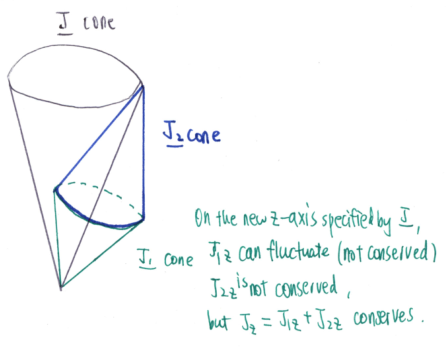
\includegraphics[width=4in]{images/qm/addition-of-momentum.png}
  \caption{Addition of Two Momentum, Conservation of z-component} \label{addition-of-momentum} 
\end{figure}



\topic{Pauli Exclusion Principle From Permutation Operator \label{section-Pauli}}
\begin{enumerate}
\item Motivate permutation operator in 2 particle system. Let's define a two-particle state vector $\ket{\Psi}$, the two particles are at $X_1, X_2$, and we define $X$ such that 
\eqn{ X =  x \otimes \{ \up, \down \} }
We cannot tell the two particles apart, thus 
\eqn{ \bra{\Psi} x_1 y_1^2 S_{1z} \ket{\Psi} = \bra{\Psi} x_2 y_2^2 S_{2z} \ket{\Psi} }
But we can permute the two particles and get different results depend on the particle property, 
\eqn{ \Psi(X_1, X_2) = e^{i \theta} \Psi(X_2, X_1) }
where
 \eqn{ \left\{ \begin{array}{ccc} \theta = \pi &  e^{i \theta} = -1 & \mbox{2 Fermions} \\ \theta = 2 \pi  & e^{i \theta} = 1 & \mbox{2 Bosons} \end{array} \right. }

\item Define a general permutation operator in multi-particle system. 
We extend this argument into many-particle system and define \textbf{a permutation operator $\hat{P}_{ij}$}, 
\eqn{ \hat{P}_{ij} \Psi(X_1, X_2, \cdots X_i, \cdots, X_j, \cdots, X_N) = \Psi (X_1, X_2, \cdots X_j, \cdots, X_i, \cdots X_N) }

Spin-statistics theorem says, 
\eqn{  P_{ij} \ket{\psi} = \left\{  
\begin{array}{cc} 
  - \ket{\psi} & \mbox{if $i,j$ are the same gene (stationary, mass, charge, I, etc), and half-integer spins (Fermion)} \\
  \ket{\psi} & \mbox{if $i,j$ are the same gene but integer spin (Boson)} \\
  \pm \ket{\psi} & \mbox{if different genes.} 
\end{array}
\right. }
That is, $\hat{P}_{ij} = \pm 1$ ($+1$ for Bosons, $-1$ for Fermions). 


\item \textbf{Proof: Pauli Exclusion Principle}. 

Assume it is possible to have two identical Fermions $X_i = X_j = X_o$, that is, 
\eqn{ \Psi (X_1, X_2, \cdots X_0, \cdots, X_0, \cdots X_N) = - \Psi (X_1, X_2, \cdots X_0, \cdots, X_0, \cdots X_N) } 
The only $\Psi$ that would satisfy the above function is $\Psi = 0$, thus \hi{two Fermions (protons, neutrons, electrons) cannot occupy the exact same spatial position and spin state.} 
\end{enumerate}




%%%%%%%%%%%%%%%% end of Fall 2012 %%%%%%%%%%%%%%%%%%%%%%%%%%%%%%%%%%%
\topic{Angular Momentum Review}
This section provides a less mathematical and more classical approach to recap some important concepts in orbital angular momentum and spin. 
\begin{enumerate}
\item Construct Cartesian Components of $\hat{L}$. 
We define the orbital angular momentum like:
\begin{align}
\hat{\uline{L}} &= \hat{\uline{r}} \cross \hat{\uline{p}} \\
\hat{\uline{L}}_x &= \hat{y} \hat{p}_z - \hat{z} \hat{p}_y = - i\hbar \left( y \ppz - z \ppy \right) \\
\hat{\uline{L}}_y &= \hat{z} \hat{p}_x - \hat{z} \hat{p}_x = - i\hbar \left( z \ppx - x \ppz \right) \\
\hat{\uline{L}}_z &= \hat{x} \hat{p}_y - \hat{y} \hat{p}_x = - i\hbar \left( x \ppy - y \ppx \right) 
\end{align}

\item Check the Components We Just Constructed. 
The question we want to ask is, `can we find the eigenvalues of each of the operators simultaneously?'

To answer the above question, we consider whether the components commute with each other. Because if $\left[ \hat{L}_x, \hat{L}_y \right] = 0$, that is to say we can pin $L_x, L_y$ at the same time. After we derive it for real (see notes), they come out to be:
\eqn{ \left[ \hat{L}_x, \hat{L}_y \right] = i \hbar ( \hat{x} \hat{P}_y - \hat{y} \hat{P}_x) = i\hbar \hat{L}_z }
\eqn{ \left[ \hat{L}_y, \hat{L}_z \right] = i \hbar ( \hat{y} \hat{P}_z - \hat{z} \hat{P}_y) = i\hbar \hat{L}_x }
\eqn{ \left[ \hat{L}_z, \hat{L}_x \right] = i \hbar ( \hat{z} \hat{P}_x - \hat{x} \hat{P}_z) = i\hbar \hat{L}_y }

That is to say, $\hat{L}_x, \hat{L}_y, \hat{L}_z$ do not have common eigenstates, and that we cannot find $L_x, L_y, L_z$ simultaneously. 

\item Define the Orbital Angular Momentum Operator $\Lhat^2$. 
What the above argument leads to is the $\hat{L}^2$,  a more physical term, and the square root of its eigenvalue is the angular momentum. 
\eqn{ \left[ \hat{L}^2, \hat{L}_x   \right] =  \left[ \hat{L}^2, \hat{L}_y   \right] =  \left[ \hat{L}^2, \hat{L}_z   \right] = 0   }
We can solve for the total angular momentum and the azimuthal component simultaneously in a coordinate system as illustrated in Figure~\ref{3DCS}. 
\begin{figure}
    \centering
    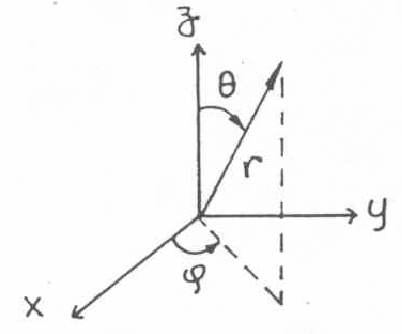
\includegraphics[width=2in]{images/qm/3DCS.png}
    \caption{Set-up of the 3D Coordinate System\label{3DCS}}
\end{figure}
\eqn{ \hat{L}_z = - i \hbar \ppphi }
\eqn{ \hat{L}^2 =  - \hbar^2 \left[ \frac{1}{\sin \theta} \pptheta \left( \sin \theta \pptheta \right) + \frac{1}{\sin^2 \theta} \ppphin2  \right] }

\item Define the Total Angular Momentum $\Jhat$:
\eqn{ \Jhat = \Lhat + \Shat }
Notice we cannot solve for the three components of $\Jhat$ simultaneously neither, because: 
\eqn{ \left[ \Jhat_x, \Jhat_y \right] &= i \hbar \Jhat_z,  &\left[ \Jhat_y, \Jhat_z \right] &= i \hbar \Jhat_x, &\left[ \Jhat_z, \Jhat_x \right] &= i \hbar \Jhat_y }


\item Eigenvalues of $\Lhat, \Jhat$. 
See Liboff 9.3 for how we get the following equations: 
\eqn{  \hat{L}^2 \phi_{l,m} (\theta, \phi) &= \hbar^2 l (l+1) \phi_{l,m} (\theta, \phi)  & \hat{L}_z \phi_{l,m} (\theta, \phi) &= \hbar m \phi_{l,m} (\theta, \phi)  }
where $l = 0,1,2, \cdots, m = -l, -l+1, \cdots, 0, \cdots l$. If we solve for $\hat{L}_x$ or $\hat{L}_y$ instead we will reach the same results as above. 

Similarly $\Jhat$ would give us:
\eqn{ \Aboxed{\Jhat^2 \phi_{l,m} (\theta, \phi) &= \hbar^2 j (j+1) \phi_{l,m} (\theta, \phi )}
& \Aboxed{ \fsp \fsp \Jhat_z \phi_{l,m} (\theta, \phi) &= \hbar m_j \phi_{l,m} (\theta, \phi ) }}
where $j = 0,1/2,1,3/2,2, \cdots, m = -j, \cdots, j$. If we solve for $\Jhat_x$ or $\Jhat_y$ instead we will reach the same results as above. 

\item Eigenfunctions $\phi_{l,m}$. The eigenfunction in the above equation, $\phi_{l,m}$, are commonly called the \textbf{Spherical Harmonics $Y_l^m (\theta, \phi)$}:
  \eqn{ Y_l^m (\theta, \phi) = \frac{1}{\sqrt{2 \pi}} e^{im\phi} P_l^m (\phi)   }
  Comments:
  \begin{itemize}
  \item $\psi( r, \theta, \phi) = R(r) Y_{lm} (\theta, \phi)$. 
  \item $\int_0^{2\pi} \dphi \int_0^{\pi} \sin \theta \dtheta |Y_{lm} (\theta, \phi) |^2 = 1.$
  \item Spherical Harmonics also implies that the unit of angular momentum is $\hbar$.
  \item Degeneracy: \textbf{For a given $l$ value, there are $2l+1$ number of degeneracy.} For instance, for $l=5$, we have 11 eigenstates $Y_5^5, Y_5^4, \cdots Y_5^{-5}$ that correspond to the same $l$, or the same $L^2 = 30 \hbar^2$. That is, for the same $L^2$, the projection onto the azimuthal plan are degenerate.  
  \item $L_z$ is not continuous. Given a $L^2$, we can draw a bunch of cones, each surface describe the superposition of possible eigenfunctions. L will never entirely align with the z axis. 
  \end{itemize}
\end{enumerate}


%%%%%%%%%%%%%%%%%%%%%%%%%%%%%% SUMMARY %%%%%%%%%%%%%%%%%%%%%%%%%%%%%%%%%%%%%%%%%%%%%%%%
\topic{Summary} 
\begin{enumerate}
\item Commutating relations: 
  \begin{enumerate}
  \item Most basic properties about angular momentum:
    \eqn{ [V_i, J_j] &= i \hbar \epsilon_{ijk} V_k}
    which leads to: $[L_x, L_y] = i \hbar L_z, [L_y, L_z] = i \hbar L_x, [L_z, L_x] = i \hbar L_y$. 
    \eqn{[J^2, \vecn \cdot J] &= 0 }

  \item Raising and lowering operators satisfy,
    \eqn{ J_+ &= J_x + i J_y & J_- &= J_x - i J_y }
    \eqn{ [J_z, J_-] &= - \hbar J_-   &J_- \ket{z} &= \alpha \ket{z-1} }

  \item Eigenvalues \& eigenvectors conclusion: 
    \eqn{ J^2 \ket{jm} &= j (j+1) \hbar^2 \ket{j m }    & J_z \ket{jm} &= m \hbar \ket{j m} }
    \eqn{ J_{\pm} \ket{jm} &= \hbar \sqrt{j(j+1) - m(m\pm 1)} \ket{jm \pm 1}  }
    \eqn{ J_x \ket{jm} &= \frac{\hbar}{2} (\sqrt{j(j+1) - m(m+1)} \ket{jm+1} + \sqrt{j(j+1) - m(m-1)} \ket{jm-1})  }
    \eqn{J_y \ket{jm} &= \frac{\hbar}{2} (-\sqrt{j(j+1) - m(m+1)} \ket{jm+1} + \sqrt{j(j+1) - m(m-1)} \ket{jm-1})  }    
  \end{enumerate}

\item Quantum numbers, 
  \begin{enumerate}
  \item $l$ (orbital): integers, $0 \le l \le n$. A subset of $j$ is the solution from orbital component. 
  \item $j$ (total): integer steps, $|l-s|, \cdots, |l+s|$. It completely construct $l$ and $s$. 
  \item $m_j$ (z-component of total): $-j, \cdots j$ (includes 0 when $j$ is an integer, and does not include 0 when $j$ is a half-integer). Its degeneracy is $2j+1$. 
  \end{enumerate}

\item Angular momemtum addition: given any two of $s, l, j$ (or given $l_1, l_2$ and solving for total $l$), we can compute the 3rd one by taking integer steps from the difference to the maximum. Example: 
  \eqn{ |s-l| &\le j \le s+l   & |s-j| &\le l \le s+j }
\end{enumerate}

\begin{table}[ht]
  \begin{tabular}{|p{1.5in}|p{1.2in}|p{1.2in}|p{1.2in}|} \hline
    & $\Lhat$ (Orbital) & $\Shat$ (Spin) &$\Jhat = \Lhat + \Shat$ (Total) \\ \hline
    \multirow{3}{*}{Commutating Relations} &
    $\left[ \Lhat_x, \Lhat_y \right] = i \hbar \Lhat_z$ &  $\left[ \Shat_x, \Shat_y \right] = i \hbar \Shat_z$ &  $\left[ \Jhat_x, \Jhat_y \right] = i \hbar \Jhat_z$ \\
    &  $\left[ \Lhat_y, \Lhat_z \right] = i \hbar \Lhat_x$ &  $\left[ \Shat_y, \Shat_z \right] = i \hbar \Shat_x$ &  $\left[ \Jhat_y, \Jhat_z \right] = i \hbar \Jhat_x$ \\
    &  $\left[ \Lhat_z, \Lhat_x \right] = i \hbar \Lhat_y$ &  $\left[ \Shat_z, \Shat_x \right] = i \hbar \Shat_y$ &  $\left[ \Jhat_z, \Jhat_x \right] = i \hbar \Jhat_y$ \\ \hline
    Quantum Numbers & $ l = 0,1,2,\cdots,n $ & $s = 0, 1/2, 1, \cdots$               & $ j =|l-s|,\cdots, |l+s|$ \\
    (all in integer steps) & $-l \le m_l \le l  $  & $ -s \le m_s \le s$  & $-j \le m_j \le j$  \\ \hline
    \multirow{2}{*}{Eigenvalues} 
    & $\expect{L^2} = \hbar^2 l (l+1)$ 
    & $\expect{S^2} = \hbar^2 s (s+1)$
    & $\expect{J^2} = \hbar^2 j(j+1)$\\ 
    & $\expect{L_z} = \hbar m_l$ 
    & $\expect{S_z} = \hbar m_s$ 
    & $\expect{J_z} =  \hbar m_j$  \\ \hline
  \end{tabular}
  \caption{Comparison of Quantum Numbers $l,s,j$} \label{quantum-numbers}
\end{table}


\textbf{Know how to add angular momentum.} 
Examples:
\begin{enumerate}
\item Find $\Lhat, \Jhat$ for 2 electrons, 1 electron, and a hydrogen atom. 

\textbf{Answer:} 
\begin{enumerate}
\item $2e^-: \Lhat = \Lhat_1 + \Lhat_2 $ 
\item $1e^-: \Jhat = \Lhat + \Shat$
\item \ce{^2H = p + n}: $l =0. \Jhat = \Shat_p + \Shat_n$. 
\end{enumerate}

\item Adding Two Orbital Momentum $\Lhat= \Lhat_1 + \Lhat_2$ of two independent systems.

\textbf{Answer:} we want to find the $(l,m)$ from the four quantum numbers $l_1, m_1, l_2, m_2$.
\begin{itemize}
\item $\Lhat^2 = (\Lhat_1 + \Lhat_2)^2 $
\item $ \Lhat_z = \Lhat_{1z} + \Lhat_{2z} \Rightarrow m_{\mathrm{max}} = m_{\mathrm{1,max}} + m_{\mathrm{2,max}} = l_1 + l_2.$
$\fsp l_{\mathrm{max}} = m_{\mathrm{max}} = l_1 + l_2.$
\item $ \mbox{Total \# of independent states } N = (2 l_1 + 1) (2l_2 + 1) = \Sum_{l_{\mathrm{min}}}^{l_{\mathrm{max}}} (2l+1) \Rightarrow l_{\mathrm{min}} = |l_2 - l_1 |.$ Thus,
\eqn{ l = |l_2 - l_1|, \cdots , l_1 + l_2}
\end{itemize}


\item Adding two electrons, given $l_1 = 1, l_2 = 2$. 

\textbf{Answer:}
\begin{itemize}
\item $l = 1,2,3$.
\item $L = \hbar \sqrt{l (l+1)} = \hbar \sqrt{2}, \hbar \sqrt{6}, \hbar \sqrt{12}.$.
\item $N = \Sum_1^3 (2l+1) = 3 + 5 + 7 = 15$, or $N = 3 \times 5 = 15$. 
\end{itemize}
\end{enumerate}


\end{document}
